\documentclass[11pt, oneside, final]{article} 
\usepackage[utf8]{inputenc} 
\usepackage{a4wide} 
\usepackage[russian]{babel} 
\usepackage{graphicx} 
\usepackage{epstopdf} 
\usepackage{amsmath} 
\usepackage{amsfonts} 
\usepackage{amssymb} 
\usepackage{amsthm}
\usepackage{epstopdf}
\usepackage{float}
\usepackage{subcaption}
\usepackage[perpage]{footmisc}
%\newtheoremstyle{mytheorem}% name of the style to be used
%  {}% measure of space to leave above the theorem. E.g.: 3pt
%  {}% measure of space to leave below the theorem. E.g.: 3pt
%  {}% name of font to use in the body of the theorem
%  {}% measure of space to indent
%  {}% name of head font
%  {:}% punctuation between head and body
%  { }% space after theorem head; " " = normal interword spacewww
%  {}% Manually specify head
%\theoremstyle{mytheorem}
\newtheoremstyle{break}%
  {}{}%
  {\itshape}{}%
  {\bfseries}{}%  % Note that final punctuation is omitted.
  {\newline}{}
\theoremstyle{break}
\newtheorem*{PMP}{Принцип Максимума Понтрягина} 
\numberwithin{equation}{section} 
\theoremstyle{plain}
\newtheorem{theorem}{Теорема}[section] 
\newtheorem{property}{Свойство}[section] 
\newtheorem{corollary}{Следствие}[theorem] 
\newtheorem{lemma}[theorem]{Лемма} 
\newtheorem*{statement}{Утверждение} 
\theoremstyle{definition}
\newtheorem{definition}{Определение}[section] 
\renewenvironment{proof}{
\noindent\textit{Доказательство: }} {\qed}
\newcounter{icount}
\graphicspath{{figures/}}
%commands
\newcommand \bitem[1][]{
\item \textbf{#1}} 
\newcommand \four[1][\lambda]{\mathfrak{F}(#1)} 
\newcommand \fft[1][\lambda]{F(#1)} 
\newcommand \rarrow{\rightarrow} 
\newcommand \real{\mathbb{R}}
\newcommand \intinf[1][{\,dt}]{ \int\limits_{-\infty}^{+\infty}{{#1}}} 
\renewcommand \qed{$\blacksquare$}
\newcommand{\scalar}[2]{\langle #1, #2\,\rangle}

\DeclareMathOperator{\sgn}{sgn}

\begin{document}

%Title
    \thispagestyle{empty}
    \begin{center}
        \ \vspace{-3cm}
    
        
\includegraphics[width=0.5
        \textwidth]{msu}\\
        {\scshape Московский государственный университет имени М.~В.~Ломоносова}\\
        Факультет вычислительной математики и кибернетики\\
        Кафедра системного анализа
    
        \vfill
    
        {\LARGE Отчёт по практикуму}
    
        \vspace{1cm}
    
        {\Huge\bfseries "<Линейная Задача Быстродействия">} 
    \end{center}

    \vspace{1cm}
    \begin{flushright}
        \large \textit{Студент 315 группы}\\
        В.\,А.~Сливинский
    
        \vspace{5mm}
    
        \textit{Руководитель практикума}\\
        к.ф.-м.н., доцент П.\,А.~Точилин 
    \end{flushright}

    \vfill
    \begin{center}
        Москва, 2018 
    \end{center}
    \pagebreak

    %Contents
    \tableofcontents

    \pagebreak


    %Task

    \section{Постановка~задачи}
    \label{sec:task}
    \subsection{Общая~формулировка~задачи} 
    \label{sub:general}
    Задана линейная система ОДУ: 
    \begin{equation} 
        \label{task:system} 
        \dot x = Ax + u + f,\:t \in [t_0, +\infty)
    \end{equation}
    Здесь, \(x, f \in \real^2, \, A \in \real^{2\times2}, \, u \in \real^2 \).
     Кроме того, на управление \( u \) наложено дополнительное ограничение \(u \in \mathcal{P} \). Пусть \( \mathcal{X}_0 \)~---~начальное множество значений фазового вектора, \( \mathcal{X}_1 \)~---~целевое множество значений фазового вектора. Для заданных множеств \( \mathcal{X}_0 ,\, \mathcal{X}_1, \, \mathcal{P} \) необходимо решить задачу быстродействия, т.е. найти минимальное время \(T > 0 \), за которое траектория системы, выпущенная в момент времени \( t_0 \) из некоторой точки множества \( \mathcal{X}_0 \), может попасть в некоторую точку множества \( \mathcal{X}_1 \). 
    \begin{gather}
        \label{task:P} 
        \mathcal{P} = p + \left\{ (x_1, x_2) \in \real^2 \, \colon 9x_1^2 + 4x_2^2 \leqslant r \right\}, \; p \in \real ^2; \\
        \label{task:X0}
        \mathcal{X}_0 = \{x_0\}; \\
        \label{task:X1}
        \mathcal{X}_1 = \left\{ x = (x_1, x_2) \in \real^2 \, \colon a(x_1 - x_{11})^2 + b |x_2 - x_{12}| \leqslant c \right\}, \; a, b, c > 0.
    \end{gather} 
    Требуется: 
    \begin{enumerate} 
        \item Написать в среде Matlab программу с пользовательским интерфейсом, которая по заданным значениям параметров \(A, f, t_0, r, p, x_0, a, b, c, x_{11}, x_{12}\) определяет, разрешима ли задача \eqref{task:system}. Если задача разрешима, программа должна (приближённо) найти значение T и построить графики компонент оптимального управления, оптимальной траектории, сопряжённых переменных. Кроме того, программа должна допускать возможность улучшения решения, как локальным, так и глобальным методами.
        \item Для различных значений параметров (в том числе, для различных собственных значений матрицы A) провести анализ системы \eqref{task:system}, численно решить задачу и построить соответствующие графики.
    \end{enumerate}
    \pagebreak
    %Formal task
    \subsection{Формальная~постановка~задачи} 
    \label{sub:formal}
    \begin{enumerate}
        \item Провести необходимые исследования системы \eqref{task:system} и привести сопутствующие теоретические выкладки;
        \item \label{enum:method} Разработать и описать численный метод решения задачи и возникающих подзадач;
        \item Реализовать на языке MATLAB программу, удовлетворяющую условиям из \ref{sub:general} и реализующую численный метод из пункта \ref{enum:method}.
        Для этого, реализовать:
        \begin{itemize}
            \item  Пользовательский интерфейс ввода исходных данных;
            \item  Алгоритм поиска управлений и траекторий, подозрительных на оптимальные, а также алгоритм отбора из них оптимальных (при наличии таковых);
            \item  Алгоритм и интерфейс построения требуемых графиков;
            \item  Алгоритм локального и глобального улучшения решения; 
            \item  Алгоритм сохранения и загрузки промежуточных данных, значений параметров и полученных ответов.
        \end{itemize}
        \item Построить, используя написанную программу, графики для различных значений параметров
    \end{enumerate}
    \pagebreak
    \section{Некоторые~необходимые~теоретические~выкладки}
    \label{sec:theory}
    \subsection{Принцип максимума} % (fold)
    \label{sub:maximum}
    Прежде всего, установим принцип максимума Понтрягина в следующей формулировке:\footnote{Доказательство приведено, например, в \cite{Pontr'yaginEtAl:maximum}}
    \begin{PMP}[В формулировке из \cite{RoublevTochilin:matlab}]
        \label{th:max}
        Пусть \((u^{*}(\cdot), x^{*}(\cdot))\)~--- оптимальная пара. \\ Тогда существует \(\psi(t) \in AC[t_0, t_1], \psi(t) \neq 0 \ \forall t \in [t_0, t_1]\!: \)
        \begin{align}
            \dot \psi =& -\!A^{T}\psi \label{eq:conj} \\
            \scalar{Bu^{*}(t)}{\psi(t)} =& \, \rho(\psi(t)|B\mathcal{P}) \label{eq:optimum} \\ 
            \scalar{\psi(t_0)}{x^{*}(t_0)} =& \, \rho(\psi(t_0)|\mathcal{X}_0) \label{eq:trans:1} \\
            \scalar{-\psi(t_1)}{x^{*}(t_1)} =& \, \rho(-\psi(t_1)|\mathcal{X}_1) \label{eq:trans:2}            
        \end{align}
    \end{PMP}
    \noindent Систему \eqref{eq:conj} называют \emph{сопряжённой системой}, её решение \(\psi = \psi(t)\)~--- \emph{сопряжёнными переменными}, а условия \eqref{eq:trans:1} и \eqref{eq:trans:2}~--- \emph{условиями трансверсальности}. Условие \eqref{eq:optimum} позволяет выделить из всех возможных управлений семейство "<подозрительных">  на оптимальные. \\
    \subsection{Исследование сопряжённой системы} % (fold)
    \label{sub:conjugate}
    Для того, чтобы однозначно определить решение системы \eqref{eq:conj}, нам необходимо присовокупить к ней некоторые начальные условия. Мы, для удобства решения, будем рассматривать \(\psi(t_0) = \psi_0\). В результате получим задачу Коши
    для сопряжённой системы:
    \begin{equation}
        \left\{
        \label{eq:cauchy}
        \begin{aligned}
            & \dot \psi(t) = -\!A^{T}\psi(t), \ t \in [t_0, t_1] \\
            & \psi(t_0) = \psi_0 
        \end{aligned}
        \right.
    \end{equation} 
    Тогда, решение этой системы представимо в виде:
    \begin{equation}
        \label{eq:psi_final}
        \psi(t) = e^{-A^{T}(t - t_0)}\psi_0
    \end{equation}
    \subsection{Выделение управлений и траекторий, "<подозрительных"> на оптимальные} % (fold)
    \label{sub:pseudo_optimum}
    Условие \eqref{eq:optimum}, в силу свойств скалярного произведения, можно переписать в следующем виде:
    \begin{equation*}
        \scalar{B^{T}\psi(t)}{u^{*}(t)} = \, \rho(B^{T}\psi(t)|\mathcal{P}) \label{eq:optimum2}  
    \end{equation*}
    В свою очередь, раскрыв определение опорной функции множества \(\mathcal{P}\) в направлении \(B^{T}\psi(t)\), окончательно получим:
    \begin{equation}
        \label{eq:optimum:final}
        \scalar{B^{T}\psi(t)}{u^{*}(t)} = \, \sup_{u(t)\in\mathcal{P}}\scalar{B^{T}\psi(t)}{u(t)}
    \end{equation}
    Заметим, что множество \(\mathcal{P}\) (см. \eqref{task:P}) есть эллипсоид \( \mathcal{E}(p, P)\), где \(P = 
    \left(\begin{smallmatrix} \frac{r}{9} & 0 \\ 0 & \frac{r}{4} \end{smallmatrix}\right)\)~--- матрица конфигурации.
    Учтём также, что \(B = E\); из \cite{Roublev:optimal:linear} известно, что решение \(u^{*}(t)\) уравнения~\eqref{eq:optimum:final} представимо в виде:
    \begin{equation}
    \label{eq:control}
        u^{*}(t) = p + \dfrac{P\psi(t)}{\sqrt{\scalar{\psi(t)}{P\psi(t)}}}
    \end{equation}
    Данное выражение корректно, так как \(\psi(t) \neq 0\) для любого допустимого \(t\), а \(P \neq 0\). Кроме того, оно показывает, что для каждого \(\psi_0\) существует единственное "<подозрительное"> на оптимальное управление. \\
    С учётом того, что множество \(\mathcal{X}_0\) состоит из одной точки (см. \eqref{task:X0}) и первого условия трансверсальности~\eqref{eq:trans:1}, любая "<подозрительная"> на оптимальную траектория \(x^{*}(t)\) выходит из точки \(x_0\), т.е. \(x^{*}(t_0) = x_0\). Тогда, подстановкой в~\eqref{task:system} недостающих значений из~\eqref{eq:control},~\eqref{eq:psi_final} и значения \(x^{*}(t_0) = x_0\) окончательно получим систему:
    \begin{equation}
        \label{eq:system_final}
        \left\{
        \begin{aligned}
            & \dot x^{*}(t) = Ax^{*}(t) + u^{*}(t) + f,\:t \in [t_0, +\infty) \\
            & x^{*}(t_0) = x_0 \\
            & u^{*}(t) = p + \dfrac{P\psi(t)}{\sqrt{\scalar{\psi(t)}{P\psi(t)}}} \\
            & \psi(t) = e^{-A^{T}(t - t_0)}\psi_0
        \end{aligned}
        \right.
    \end{equation}
    Решение данной системы \(x^{*}(t)\) есть траектория, "<подозрительная"> на оптимальную, соответствующая управлению \(u^{*}(t)\) из \eqref{eq:control}. Заметим, что и это управление \(u^{*}(t)\), и соответствующая ему траектория \(x^{*}(t)\) однозначно определяются (при фиксированных параметрах из \ref{sub:general}) лишь значением \(\psi(t_0) = \psi_0\).
    \subsection{Оценка погрешности} % (fold)
    \label{sub:right_trans}
    Поскольку численное решение задачи сопряжено с погрешностью, требуется ввести некоторую меру погрешности условия трансверсальности на правом конце~\eqref{eq:trans:2}: оно равносильно сонаправленности вектора \(-\psi(t_1)\) и вектора внешней единичной нормали к границе множества \(\mathcal{X}_1\) в точке \(x^{*}(t_1)\).
    Множество \(\mathcal{X}_1\) представляет собой область, заключённую внутри двух парабол; для удобства, перепишем~\eqref{task:X1} в следующем виде:
    \[
        \mathcal{X}_1 = \left\{ x = (x_1, x_2) \in \real^2 \, \colon \dfrac{a}{b}(x_1 - x_{11})^2 - (\dfrac{c}{b} - x_{12})\leqslant x_2 
        \leqslant x_{12} + \dfrac{c}{b} - \dfrac{a}{b}(x_1 - x_{11})^2 \right\}, \; a, b, c > 0.
    \]
    Отсюда явно видно, что эти две параболы пересекаются в точках \(\left(x_{11} \pm \sqrt{\frac{c}{a}}, \: x_{12} \right)\)\\
    Уравнение касательной к верхней параболе в точке \(\left(x_1^0, x_2^0\right)\)\footnote{Здесь и далее, по понятным причинам, предполагаем, что точка \(\left(x_1^0, x_2^0\right)\) принадлежит границе множества \(\mathcal{X}_1\)}:
    \begin{align*}
        & x_2 - x_2^0 = -\dfrac{2a}{b}(x_1^0 - x_{11})(x_1 - x_1^0) \\
        & \dfrac{2a}{b}(x_1^0 - x_{11})(x_1 - x_1^0) + (x_2 - x_2^0) = 0;
    \end{align*}
    Отсюда, вектор нормали \(\vec n_u\) и единичной нормали \(\vec \nu_u\) к верхней параболе в точке \(\left(x_1^0, x_2^0\right)\):
    \begin{align*}
        &\vec n_u = \left( \dfrac{2a}{b} (x_1^0 - x_{11}), \: 1 \right) \\
        &\vec \nu_u = \dfrac{\vec n}{\|n\|}
    \end{align*}
    Аналогично, для нижней параболы имеем:
    \begin{align*}
        &\vec n_l = \left( \dfrac{2a}{b} (x_1^0 - x_{11}), \: -1 \right) \\
        &\vec \nu_l = \dfrac{\vec n}{\|n\|}
    \end{align*}
    Таким образом, запишем общую формулу для внешней нормали к границе множества \(\mathcal{X}_1\) в точке \(\left(x_1^0, x_2^0\right)\), при условии, что \(\left(x_1^0, x_2^0\right) \neq \left(x_{11} \pm \sqrt{\frac{c}{a}}, \: x_{12} \right)\):
    \begin{equation}
        \label{eq:normal}
        \vec n =
        \begin{cases}
            \left( \dfrac{2a}{b} (x_1^0 - x_{11}), \: 1 \right)& \text{если } x_2^0 > x_{12} \\
            \left( \dfrac{2a}{b} (x_1^0 - x_{11}), \: -1 \right)& \text{если } x_2^0 < x_{12}
        \end{cases}
    \end{equation}
    Отметим, что в точках пересечения парабол \(\left(x_{11} \pm \sqrt{\frac{c}{a}}, \: x_{12} \right)\) граница множества \(\mathcal{X}_1\) не является гладкой, следовательно, существует целый сектор направлений, по которым выполняется условие~\eqref{eq:trans:2}. \\
    В качестве меры погрешности в случае, если \(x^{*}(t_1) = \left(x_{11} \pm \sqrt{\frac{c}{a}}, \: x_{12} \right)\) возьмём модуль синуса угла между \(-\psi(t_1) \) и вектором внешней нормали к границе \eqref{eq:normal}, а если \(x^{*}(t_1) = \left(x_{11} \pm \sqrt{\frac{c}{a}}, \: x_{12} \right)\)\footnote{При решении в числах, это равенство равносильно тому, что точка \(x^{*}(t_1)\) лежит в некоторой достаточно малой окрестности точки пересечения парабол}~--- модуль синуса угла отклонения от соответстующего сектора "<нормалей"> (или 0, если \(-\psi(t_1)\) лежит в этом секторе). Для нахождения модуля синуса угла между векторами воспользуемся основным тригонометрическим тождеством, и тем фактом, что для векторов \(- \vec\psi(t_1) \text{ и } \vec n  \) косинус угла \(\varphi\) между ними равен: 
    \[\cos\varphi = \dfrac{\scalar{- \vec\psi(t_1)}{\vec n}}{\|-\psi(t_1)\| \|n\|}, \]
    откуда 
    \[\sin\varphi = \sqrt{1 - \left(\dfrac{\scalar{- \vec\psi(t_1)}{\vec n}}{\|-\psi(t_1)\| \|n\|}\right)^2}.\]
    \pagebreak
    \section{Описание~численного~метода} % (fold)
    \label{sec:method}
    \begin{enumerate}
        \item Задаём все параметры системы (загрузкой или вводом с клавиатуры), длину временного интервала \(T\), инициализируем конфигурационную матрицу эллипса \(\mathcal{P}\), соответствующие функции для множества \(\mathcal{X}_1\), функцию попадания во множество \(\mathcal{X}_1\);
        \item Проверяем, не находится ли точка \(x_0\) во множестве \(\mathcal{X}_1\) изначально;
        \item Для решения сопряжённой системы используется функция \texttt{solveConj} со следующей спецификацией: 
        \begin{verbatim}
function [ tMaj, tRet, xMaj, psi0Maj, alphaMaj, xSusp ] = solveConj( tMaj, ...
A, f, p, P, x0, t0, T, alphaSpace, opts )
        \end{verbatim} 
        \item В отдельной функции \texttt{solveConj} на единичной сфере перебираем всевозможные значения \(\psi_0 = \left( \sin(\alpha),\:\cos(\alpha)\right)^T\), рассматривая \(\alpha\) на сетке \texttt{alphaSpace}. Для каждого значения \(\psi_0\) решаем сопряженную систему при помощи функции \texttt{ode45}, реализующей метод Рунге-Кутты четвёртого порядка с параметром \texttt{events}, соответствующим функции попадания во множество \(\mathcal{X}_1\);
        \item В случае попадания во множество \(\mathcal{X}_1\) за отведённое время, фиксируем данное время как оптимальное, если оно меньше предыдущего минимума (в начале алгоритма полагаем это время равным переданному в \texttt{solveConj} значению параметра \texttt{tMaj}, при первом запуске~--- \(+\infty\)), сохраняем соответствующие этому времени значения \(\psi_0,\:x^*(t), \: \alpha^*\);
        \item Таким образом, функция \texttt{solveConj} либо возвращает в качестве оптимального времени \(+\infty\), что соответствует случаю отсутствия решения (на данной сетке), либо возвращает набор, состоящий из оптимального времени \(t^*\), оптимальной траектории \(x^*(t)\), оптимального начального условия для сопряжённой системы \(\psi_0\) и соответствующего ему угла \(\alpha^*\), а также коллекцию тестовых ("<подозрительных">) траекторий \texttt{xSusp}; по этим данным однозначно восстанавливается оптимальное управление \(u^*(t)\) и значение сопряжённых переменных \(\psi(t_1)\);
        \item Ошибка второго условия трансверсальности рассчитывается согласно пункту~\ref{sub:right_trans} в функции \texttt{calcError};
        \item Производится построение графиков согласно требованиям;
        \item При необходимости, повторно вызвав функцию \texttt{solveConj} c параметром \texttt{tMaj} равным оптимальному времени \(t^*\), полученному на предыдущем шаге, можно осуществить локальное или глобальное улучшение решения. Для локального улучшения подаём на вход функции (параметр \texttt{alphaSpace}) разбиение некоторой окрестности \(\alpha^*\), а для глобального ~--- сетку большего размера
    \end{enumerate}
    \pagebreak
    % section method (end)
    \section{Примеры}
    \subsection{Локальное и глобальное улучшение}
    \(A = \begin{bmatrix} -0.2 & 0.2 \\ 0.8 & 0.4 \end{bmatrix},\:f = \begin{bmatrix} 0 \\ 0 \end{bmatrix},\: a = 1,\: b = 1,\: c = 2,\: x_{11} = 2,\: x_{12} = 4,\: x_0 =  \begin{bmatrix} 0 \\ 1 \end{bmatrix}, \: r = 2, \\ p = \begin{bmatrix} 0 \\ -0.5 \end{bmatrix}, \: t_0 = 0, \: T = 2, \: \mathtt{gridsize} = 50 \)\\
    Cобственные значения матрицы \(A\): \(\lambda_1 = -0.4, \: \lambda_2 = 0.6\)\\
    Результат работы программы: 
    \begin{verbatim}
        Optimal time: 1.7809
        Error: 0.17255
    \end{verbatim}
    \begin{figure}[H]
        \centering
        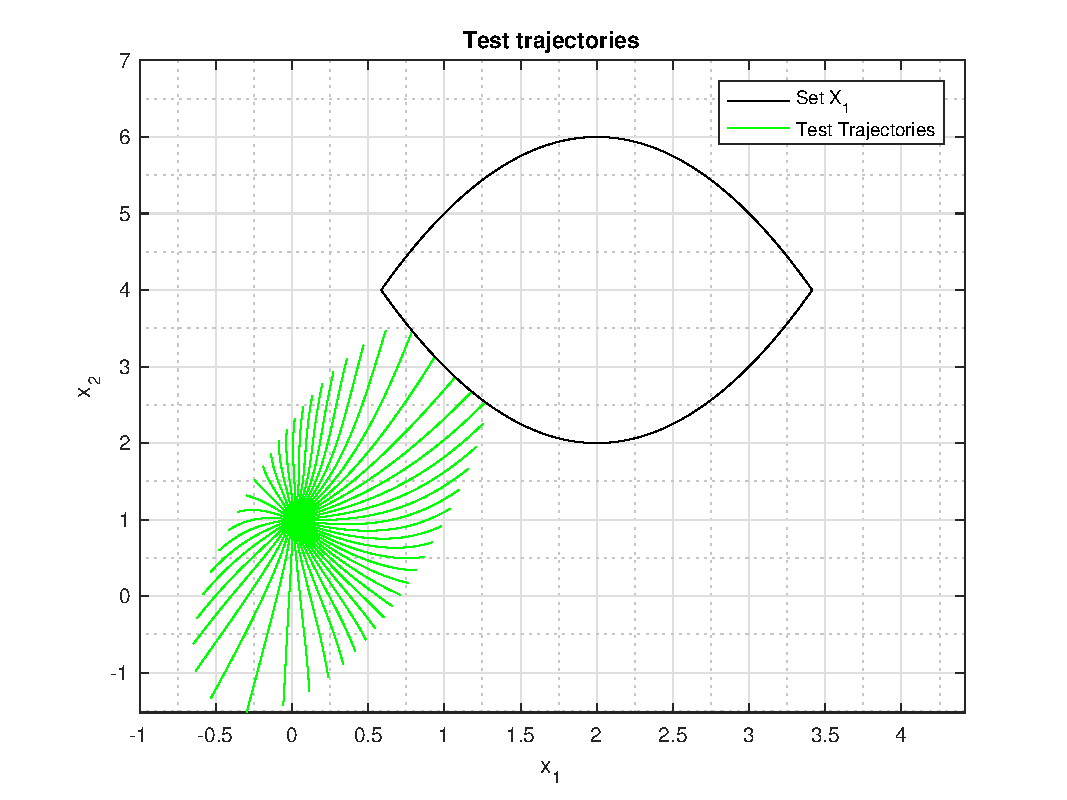
\includegraphics[width=\linewidth]{s1fig1}
        \label{pic:s1:1}
        \caption{Тестовые траектории}
    \end{figure} 
    Таким образом, до улучшения \(t^*_1 = 1.7809 \), ошибка имеет порядок \(1.7 \cdot 10^{-1}\).\\
    Проведём локальное улучшение: в окрестности угла \(\alpha^*\) построим сетку вдвое меньшего размера \(\mathtt{gridsize} / 2\). \\
    \pagebreak
    \noindent Новый результат работы программы:  
    \begin{verbatim}
        Improved optimal time: 1.7747
        Error: 0.021635
    \end{verbatim}
    После локального улучшения, \(t^*_2\) изменилось на величину порядка \(5 \cdot 10^{-3}\), а вот ошибка уменьшилась на порядок, до величины \(2 \cdot 10^{-2}\). \\
    \begin{figure}[H]
        \centering
        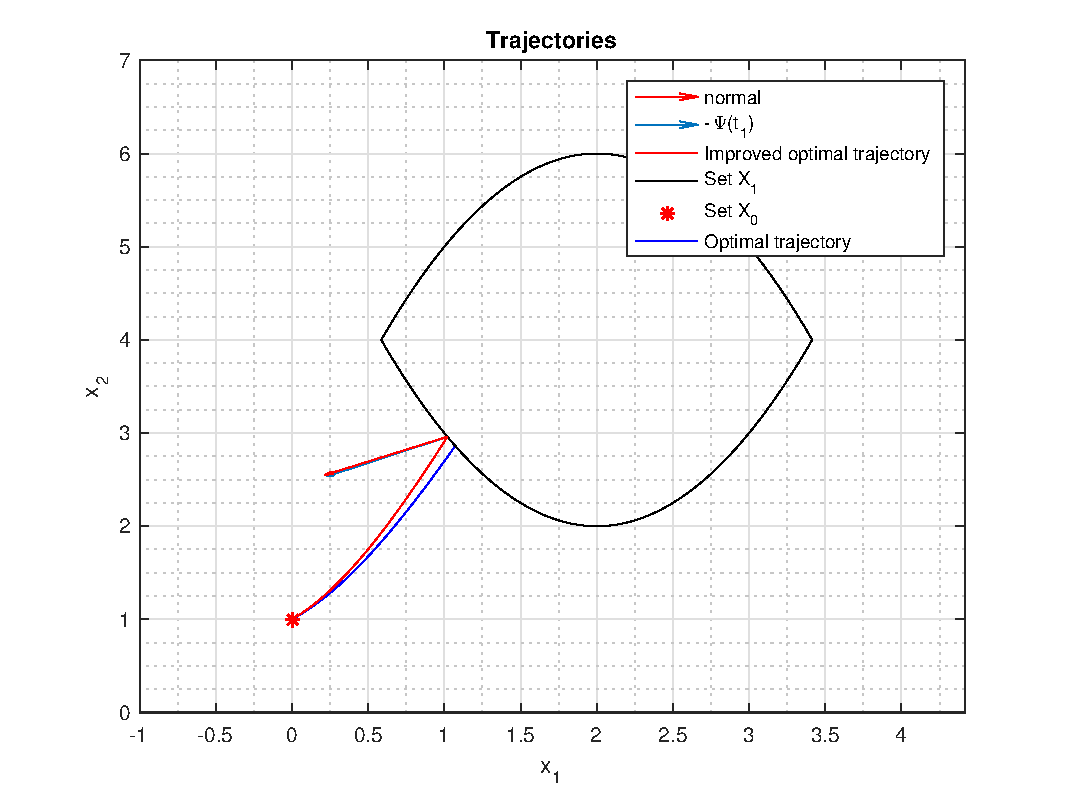
\includegraphics[width=\linewidth]{s1fig2}
        \label{pic:s1:2}
        \caption{Траектории после локального улучшения}
    \end{figure}
    \noindent
    Теперь, проведём глобальное улучшение независимо от локального: запустим программу на вдвое большей сетке, но с мажорантой \(t^*_1 = 1.7809 \), полученной про первоначальном запуске. Результат работы:
    \begin{verbatim}
        Improved optimal time: 1.7766
        Error: 0.11483
    \end{verbatim}
    \begin{figure}[H]
        \centering
        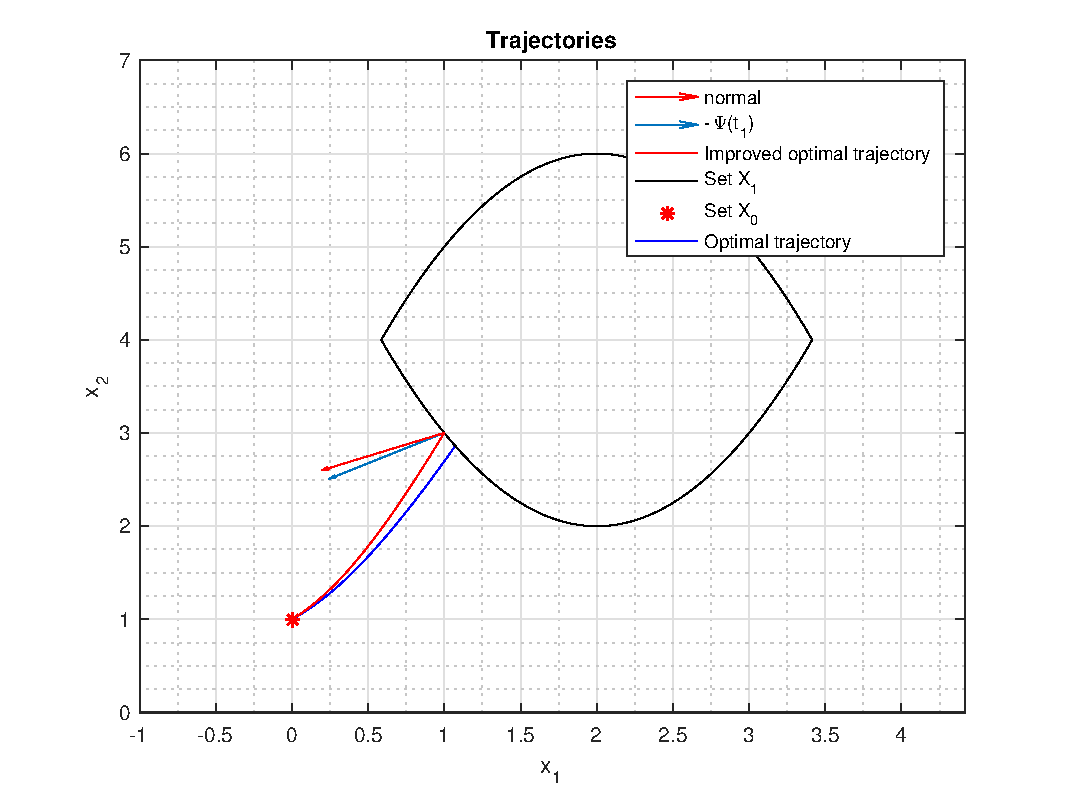
\includegraphics[width=\linewidth]{s1fig3}
        \label{pic:s1:3}
        \caption{Траектории после глобального улучшения}
    \end{figure} 
    В данном случае, локальное улучшение эффективнее, чем глобальное, так как даёт меньшее время и меньшую ошибку.
    \pagebreak
    \subsection{Неоднородная система}
    \(A = \begin{bmatrix} 1 & 0 \\ 0 & 1 \end{bmatrix},\:f = \begin{bmatrix} -0.5 \\ 0.5 \end{bmatrix},\: a = 1,\: b = 1,\: c = 1,\: x_{11} = -1.5,\: x_{12} = 2,\: x_0 =  \begin{bmatrix} 0 \\ 0 \end{bmatrix}, \: r = 3, \\ p = \begin{bmatrix} 0 \\ 0 \end{bmatrix}, \: t_0 = 0, \: T = 1, \: \mathtt{gridsize} = 72 \)\\
    Cобственные значения матрицы \(A\): \(\lambda_{1, 2} = 1\)\\
    Результат работы программы: 
    \begin{verbatim}
        Optimal time: 0.78886
        Error: 0.054337
    \end{verbatim}
    \begin{figure}[H]
            \centering
            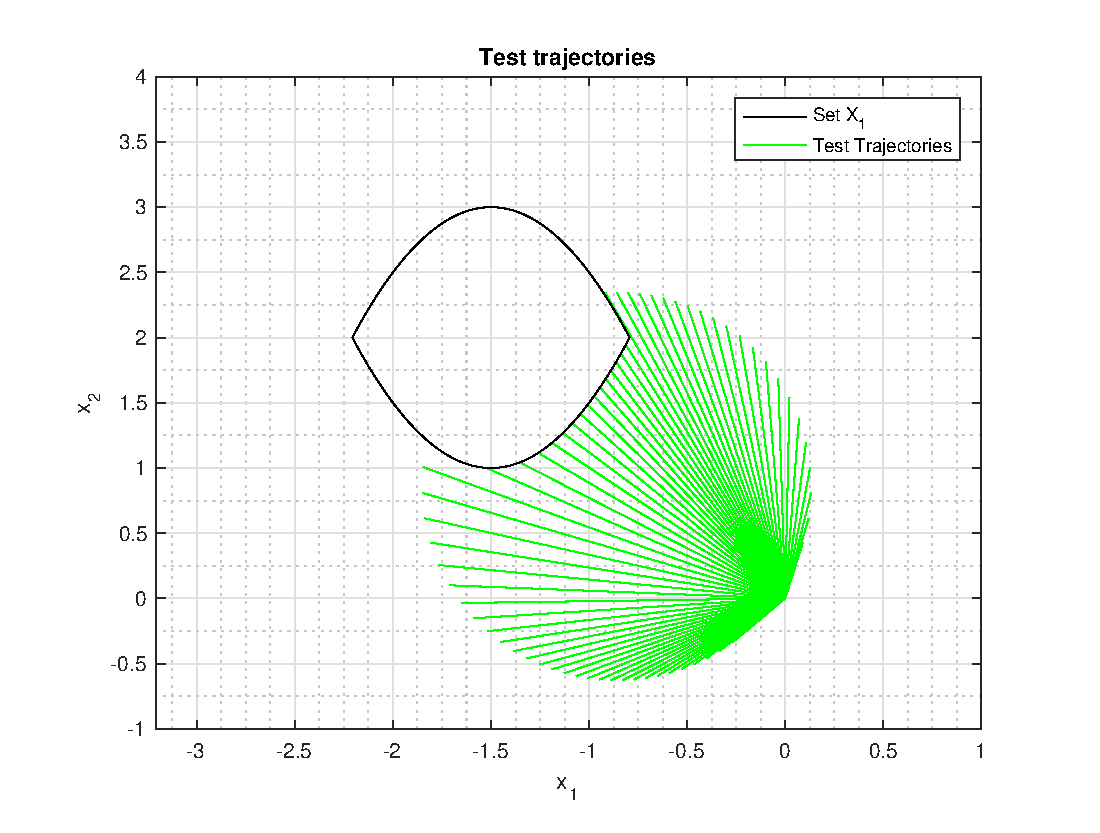
\includegraphics[width=\linewidth]{s2fig1}
            \label{pic:s2:1}
            \caption{Тестовые траектории}
    \end{figure}
    \begin{figure}[H]
            \centering
            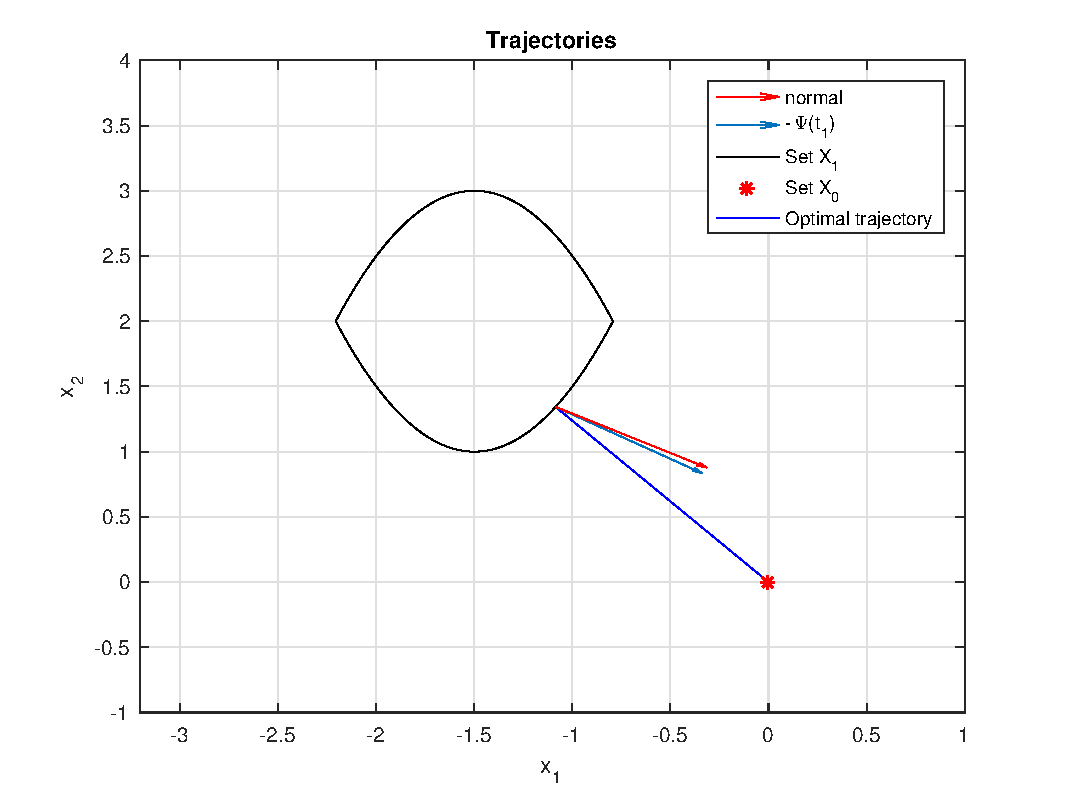
\includegraphics[width=\linewidth]{s2fig2}
            \label{pic:s2:2}
            \caption{Оптимальная траектория}
    \end{figure}
    \begin{figure}[H]
        \begin{subfigure}{0.5\linewidth}
            \centering
            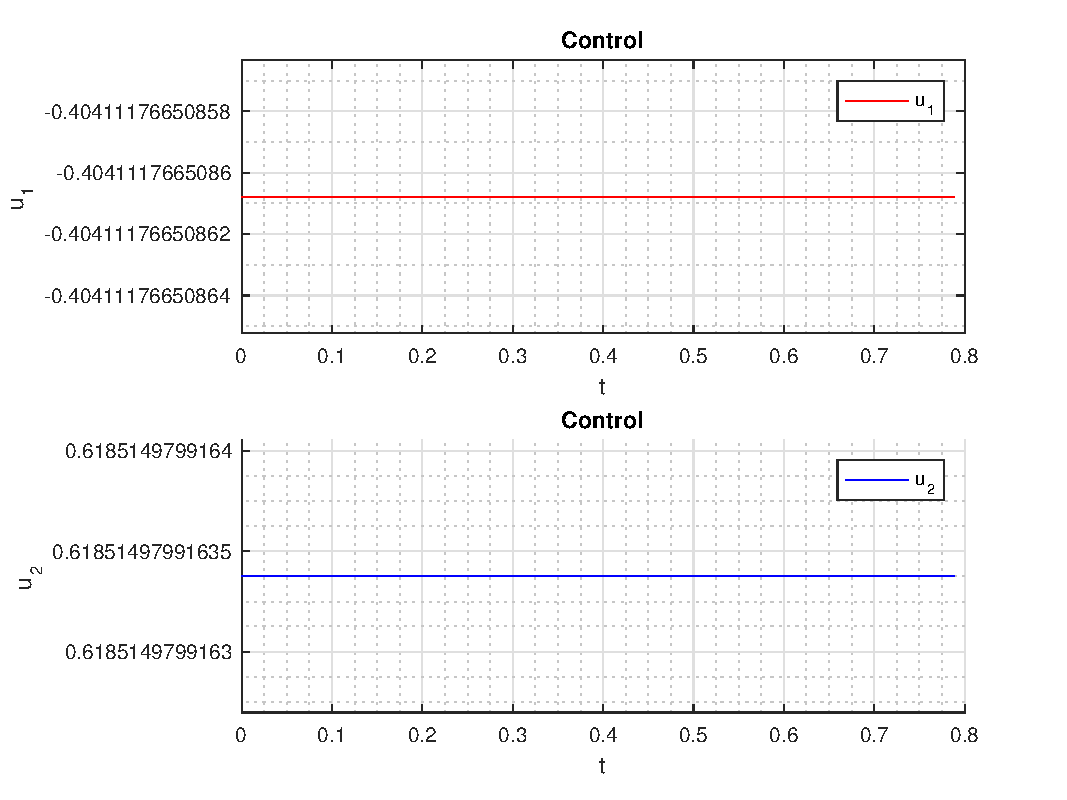
\includegraphics[width=\linewidth]{s2fig3}
            \label{pic:s2:3}
            \caption{Компоненты оптимального управления}
        \end{subfigure}
        \begin{subfigure}{0.5\linewidth}
            \centering
            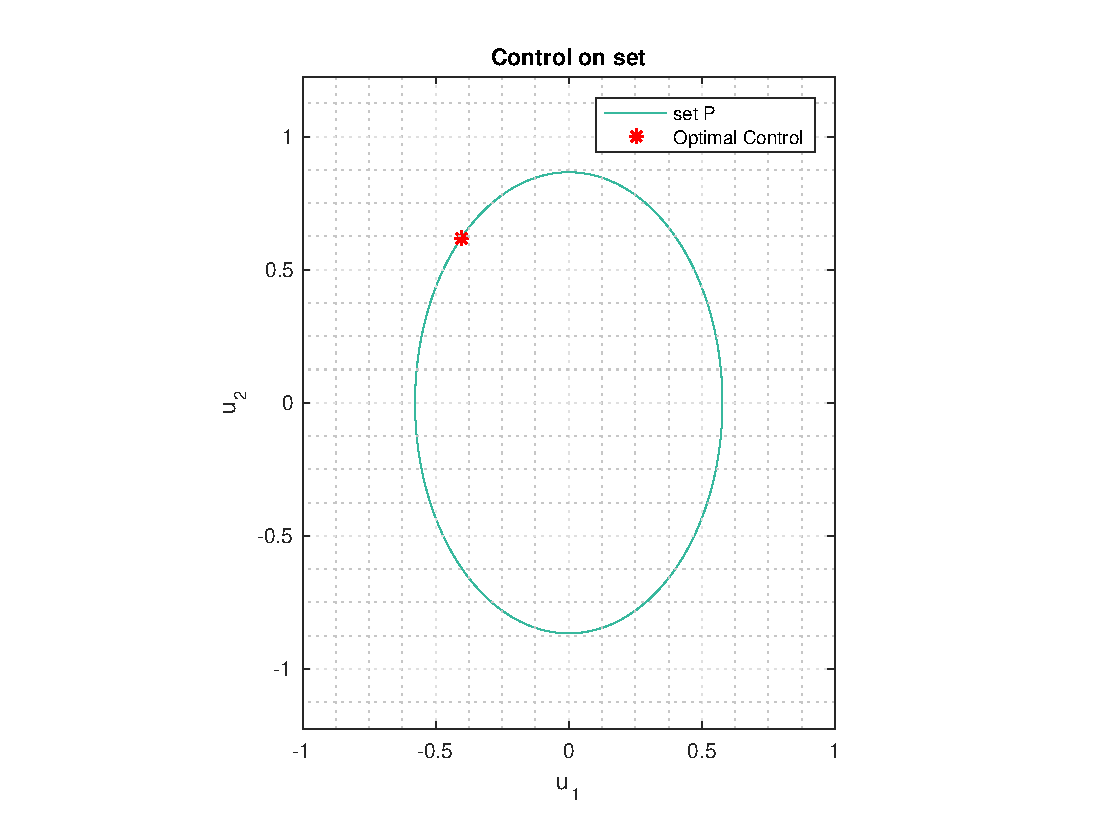
\includegraphics[width=\linewidth]{s2fig4}
            \label{pic:s2:4}
            \caption{Оптимальное управление на множестве \(\mathcal{P}\)}
        \end{subfigure}
        \caption{Оптимальное управление}
    \end{figure}
    \begin{figure}[H]
        \begin{subfigure}{0.5\linewidth}
            \centering
            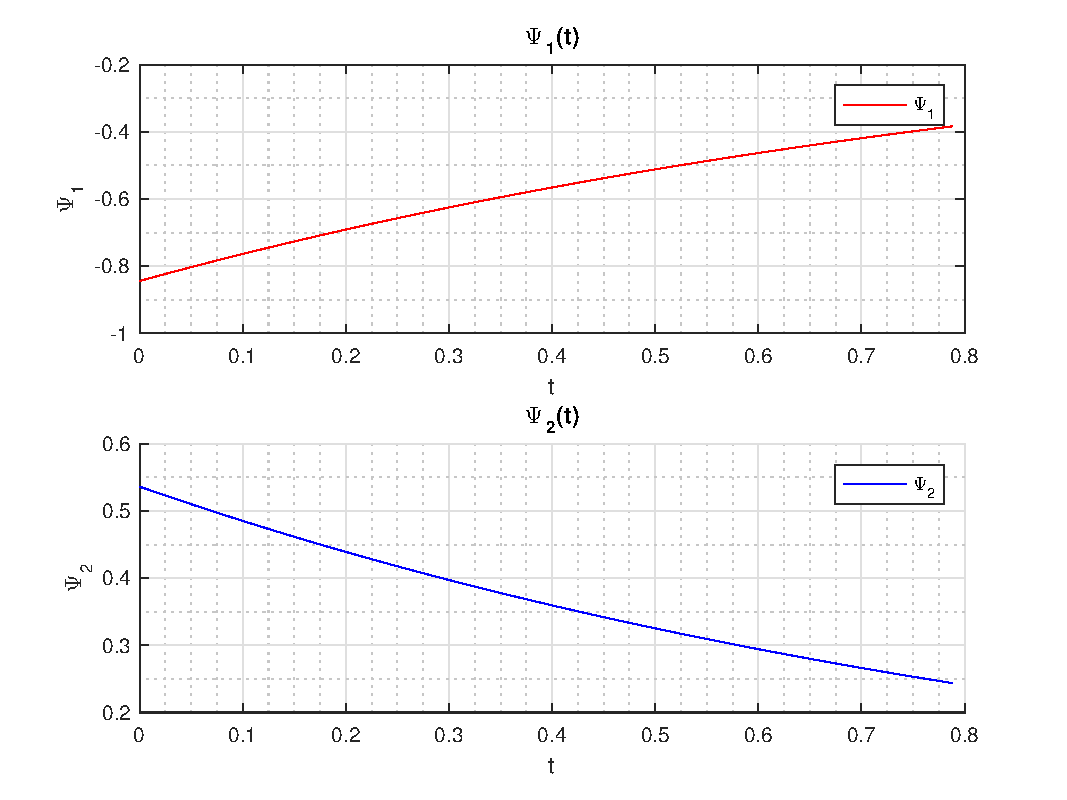
\includegraphics[width=\linewidth]{s2fig5}
            \label{pic:s2:5}
            \caption{Компоненты сопряжённых переменных}
        \end{subfigure}
        \begin{subfigure}{0.5\linewidth}
            \centering
            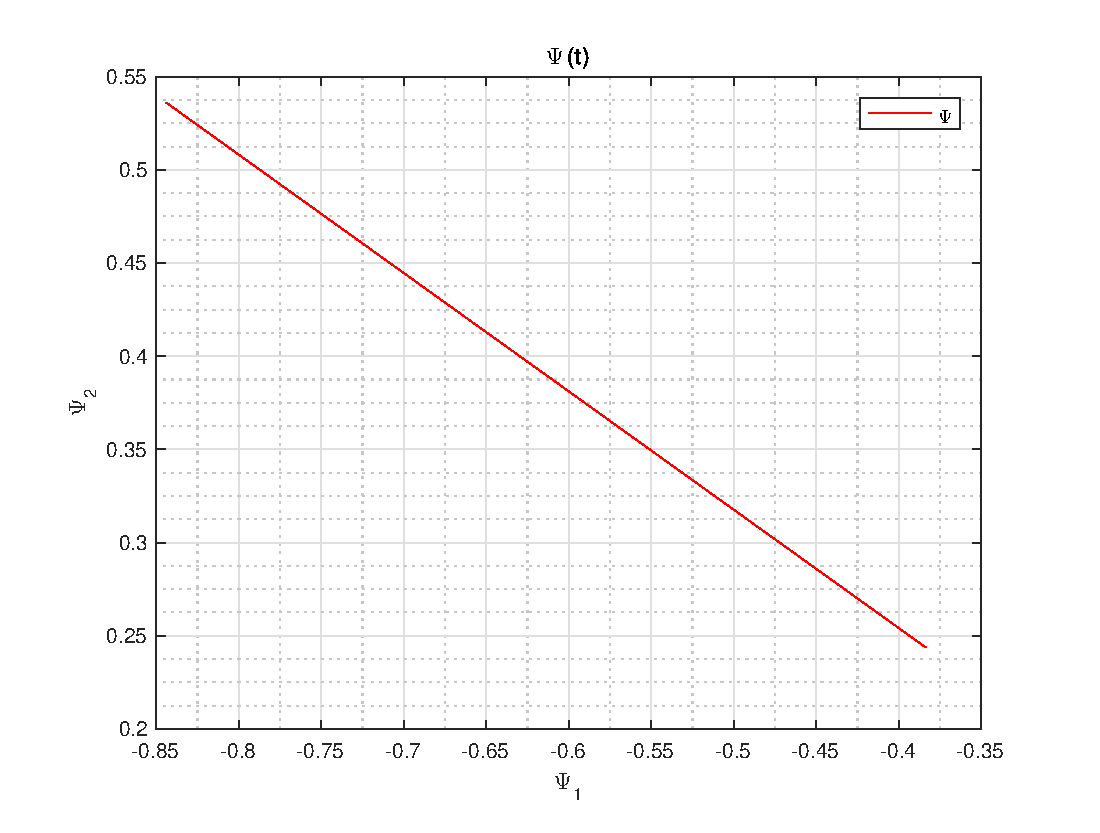
\includegraphics[width=\linewidth]{s2fig6}
            \label{pic:s2:6}
            \caption{Траектория сопряжённой системы}
        \end{subfigure}
        \caption{Сопряжённые переменные}
    \end{figure}
    \pagebreak
    \subsection{Разрыв по времени}
    \(A = \begin{bmatrix} 0 & 0 \\ 0 & 1 \end{bmatrix},\:f = \begin{bmatrix} 0 \\ 0 \end{bmatrix},\: a = 2,\: b = 1,\: c = 1,\: x_{11} = 2.028,\: x_{12} = 2,\: x_0 =  \begin{bmatrix} 0 \\ 0 \end{bmatrix}, \: r = 3, \\ p = \begin{bmatrix} 0 \\ 0 \end{bmatrix}, \: t_0 = 0, \: T = 3, \: \mathtt{gridsize} = 100 \)\\
    Cобственные значения матрицы \(A\): \(\lambda_1 = 0, \: \lambda_2 = 1\)\\
    Результат работы программы: 
    \begin{verbatim}
        Optimal time: 2.3461
        Error: 0
    \end{verbatim}
    Теперь, сдвинем множество \(\mathcal{X}_1\): положим \(x_{11} = 2.029\). Снова запустим программу:
    \begin{verbatim}
        Optimal time: 2.4638
        Error: 0.35233
    \end{verbatim}
    Как можно заметить, при сдвиге множества на величину порядка \(10^{-3}\), оптимальное время изменилось на величину большего порядка (\(10^{-1}\)). Кроме того, возросла и ошибка. Приведём, в заключение, графики оптимальных траекторий в обоих случаях:
    \begin{figure}[H]
        \begin{subfigure}{0.5\linewidth}
            \centering
            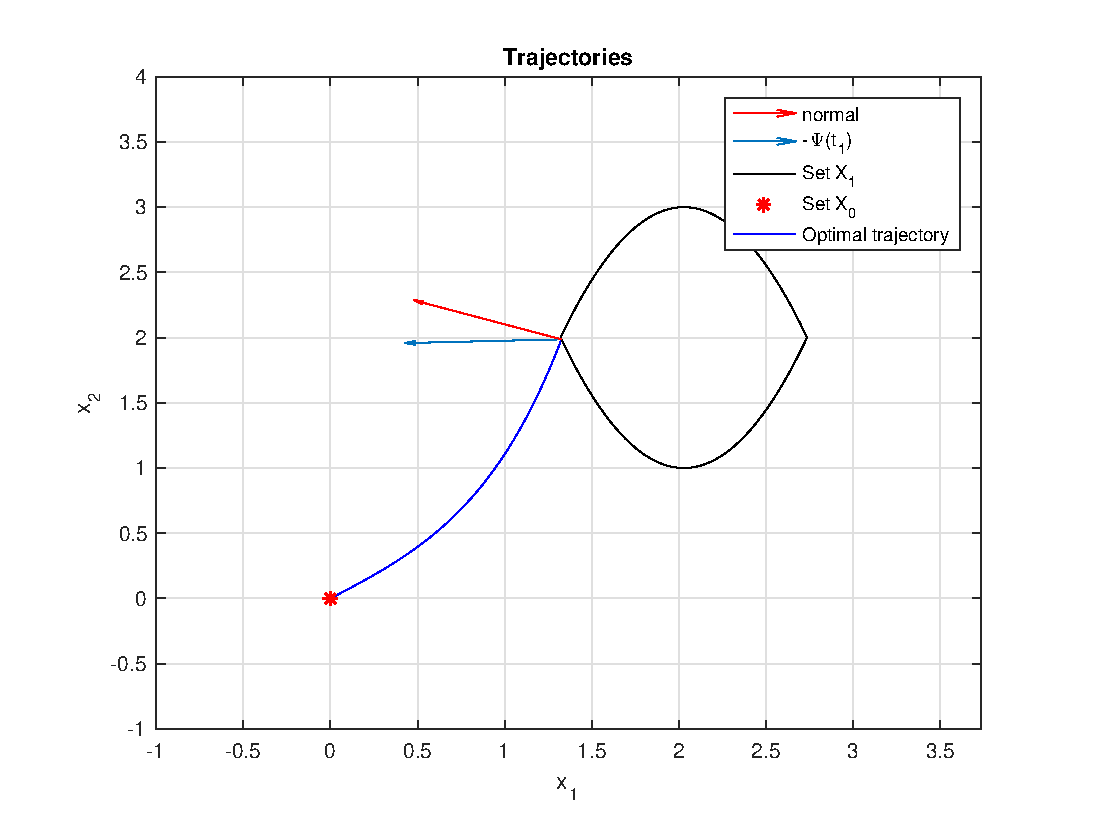
\includegraphics[width=\linewidth]{s3fig1}
            \label{pic:s3:1}
            \caption{\(x_{11} = 2.028\)}
        \end{subfigure}
        \begin{subfigure}{0.5\linewidth}
            \centering
            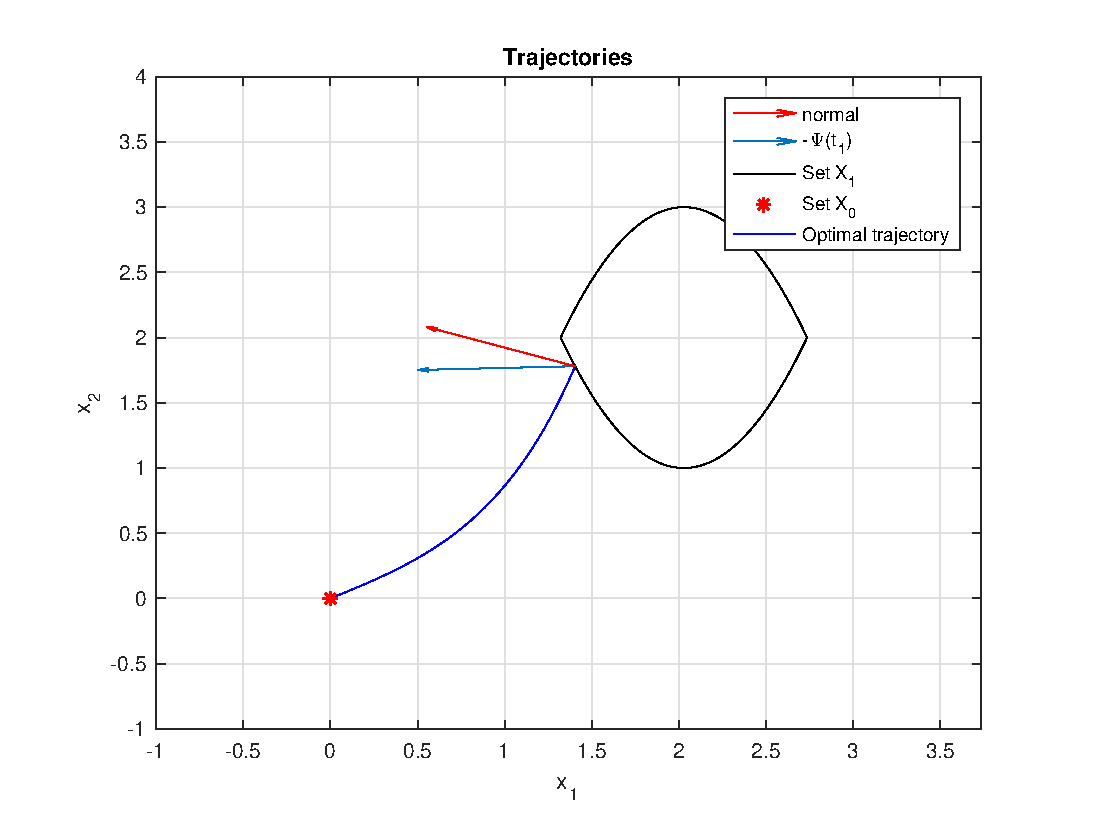
\includegraphics[width=\linewidth]{s3fig2}
            \label{pic:s3:2}
            \caption{\(x_{11} = 2.029\)}
        \end{subfigure}
        \caption{Оптимальная траектория}
    \end{figure} 
    \noindent В первом случае, траектория попадает в точку границы множества \(\mathcal{X}_1\), в которой нарушается гладкость; при этом, вектор сопряженных переменных \(-\vec\psi(t_1)\) попадает в сектор нормалей, вследствие чего удовлетворяет условию трансверсальности \eqref{eq:trans:2}.
    \pagebreak
    \subsection{Система с вырожденной матрицей}
    \(A = \begin{bmatrix} -1 & -1 \\ 0 & 0 \end{bmatrix},\:f = \begin{bmatrix} 0 \\ 0 \end{bmatrix},\: a = 2,\: b = 1,\: c = 1,: x_{11} = -1.5,\: x_{12} = 2,\: x_0 =  \begin{bmatrix} 4 \\ 2 \end{bmatrix}, \: r = 5, \\ p = \begin{bmatrix} 0 \\ 0 \end{bmatrix}, \: t_0 = 1, \: T = 2.5, \: \mathtt{gridsize} = 70 \)\\
    Cобственные значения матрицы \(A\): \(\lambda_1 = -1, \: \lambda_2 = 0\)\\
    Запустим программу и проведём одно локальное улучшение. Результат работы программы:
    \begin{verbatim}
        Optimal time: 2.2033
        Error: 0.029728
        Improved optimal time: 2.2029
        Error: 0.00038871
    \end{verbatim}
    Отметим, что выдаваемое программой время это конечное значение времени \(t_1\), а не величина \(t_1 - t_0\), характеризующая длительность перехода. В предыдущих примерах, так как \(t_0 = 0\), эти две величины совпадали.
    \begin{figure}[H]
            \centering
            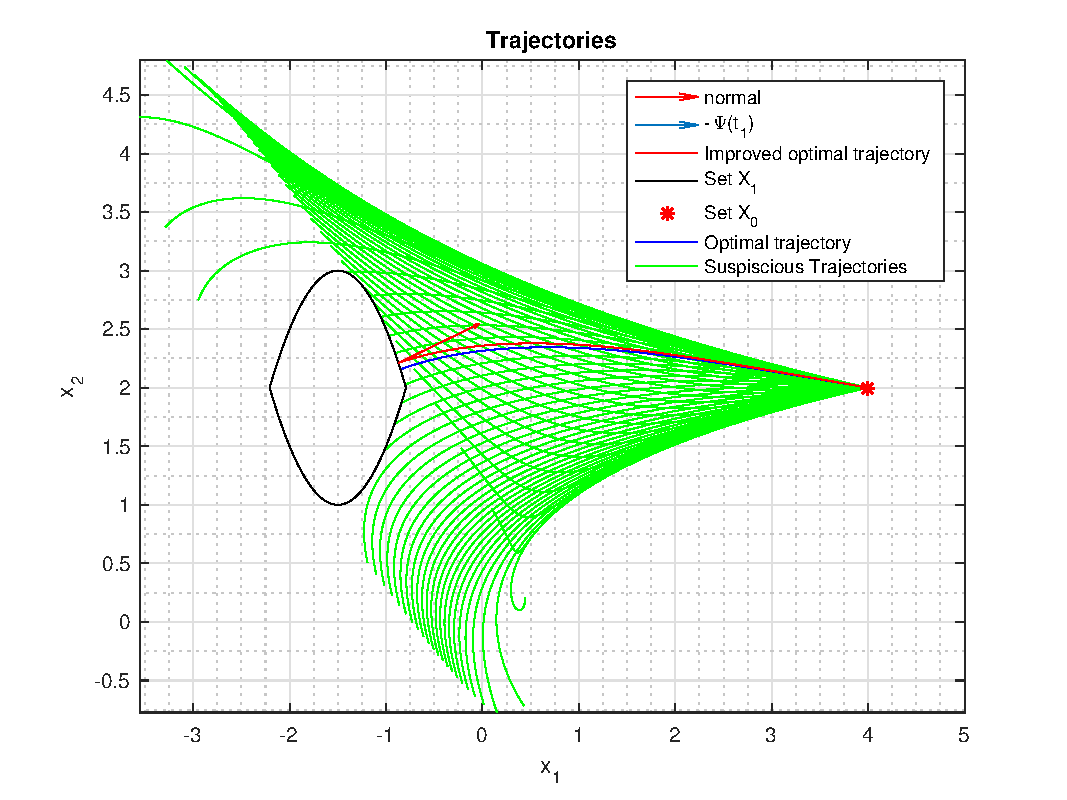
\includegraphics[width=\linewidth]{s4fig1}
            \label{pic:s4:1}
            \caption{Траектории системы (тестовые, оптимальная и улучшенная оптимальная)}
    \end{figure}
    \begin{figure}[H]
            \centering
            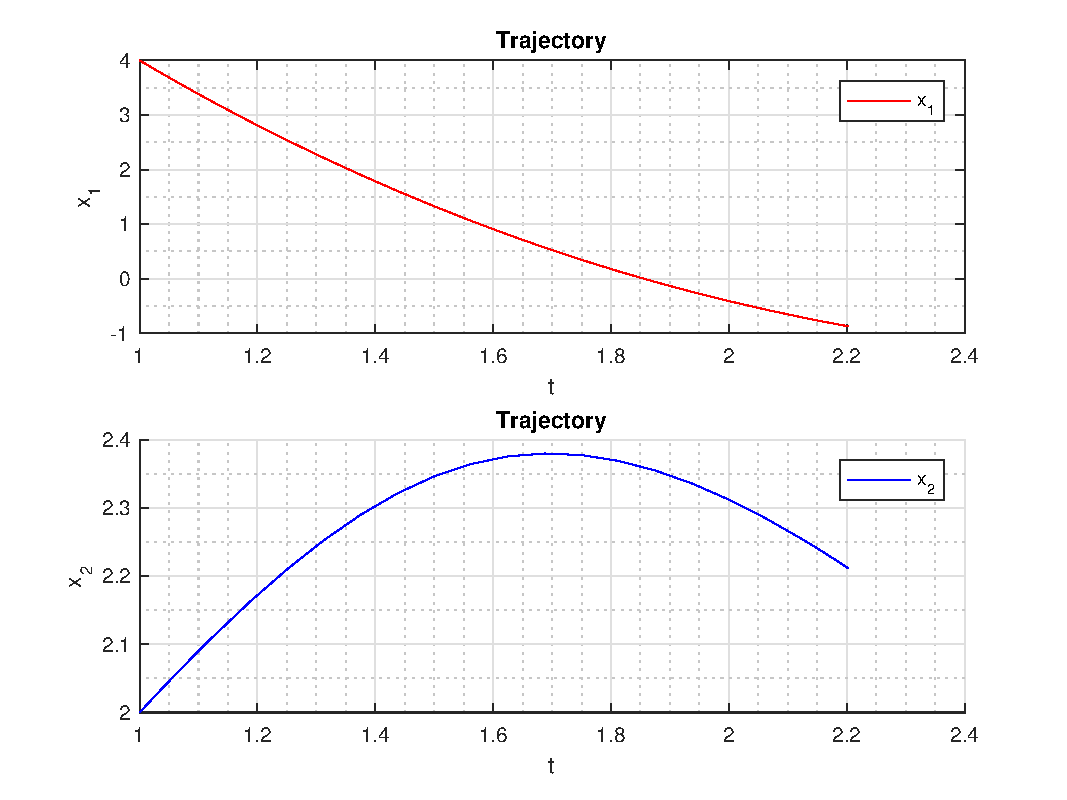
\includegraphics[width=\linewidth]{s4fig2}
            \label{pic:s4:2}
            \caption{Компоненты улучшенной оптимальной траектории}
    \end{figure}
    
    \begin{figure}[H]
        \begin{subfigure}{0.5\linewidth}
            \centering
            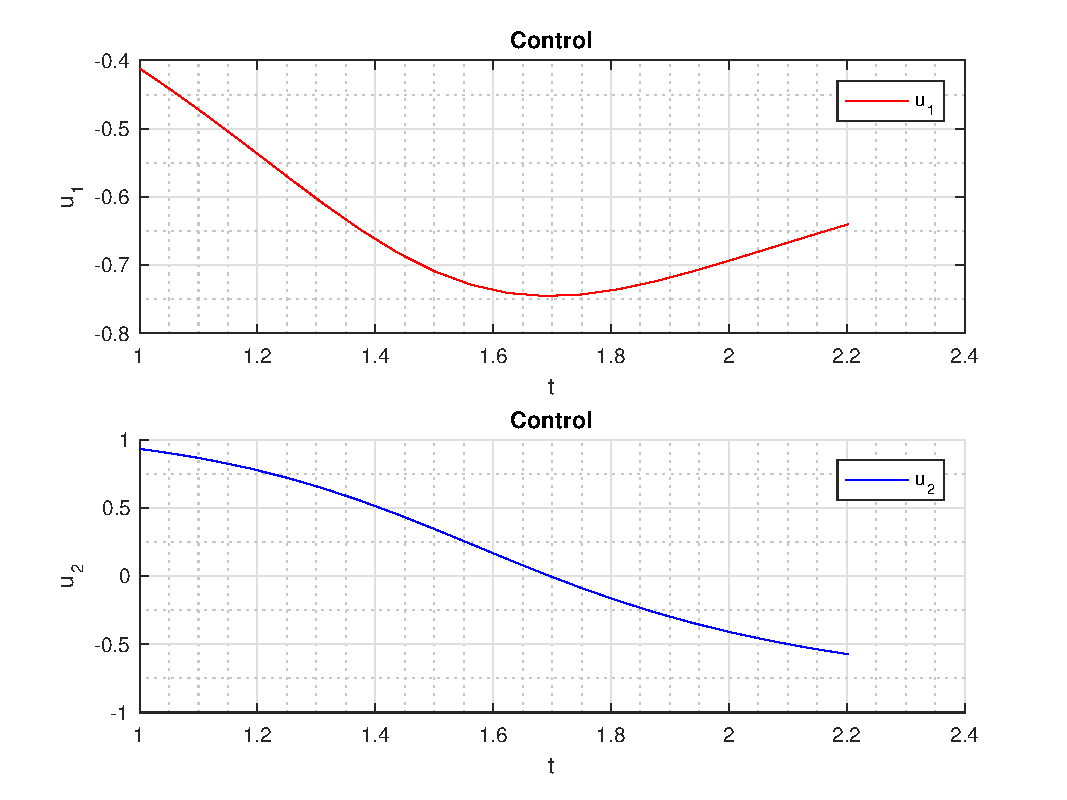
\includegraphics[width=\linewidth]{s4fig3}
            \label{pic:s4:3}
            \caption{Компоненты оптимального управления}
        \end{subfigure}
        \begin{subfigure}{0.5\linewidth}
            \centering
            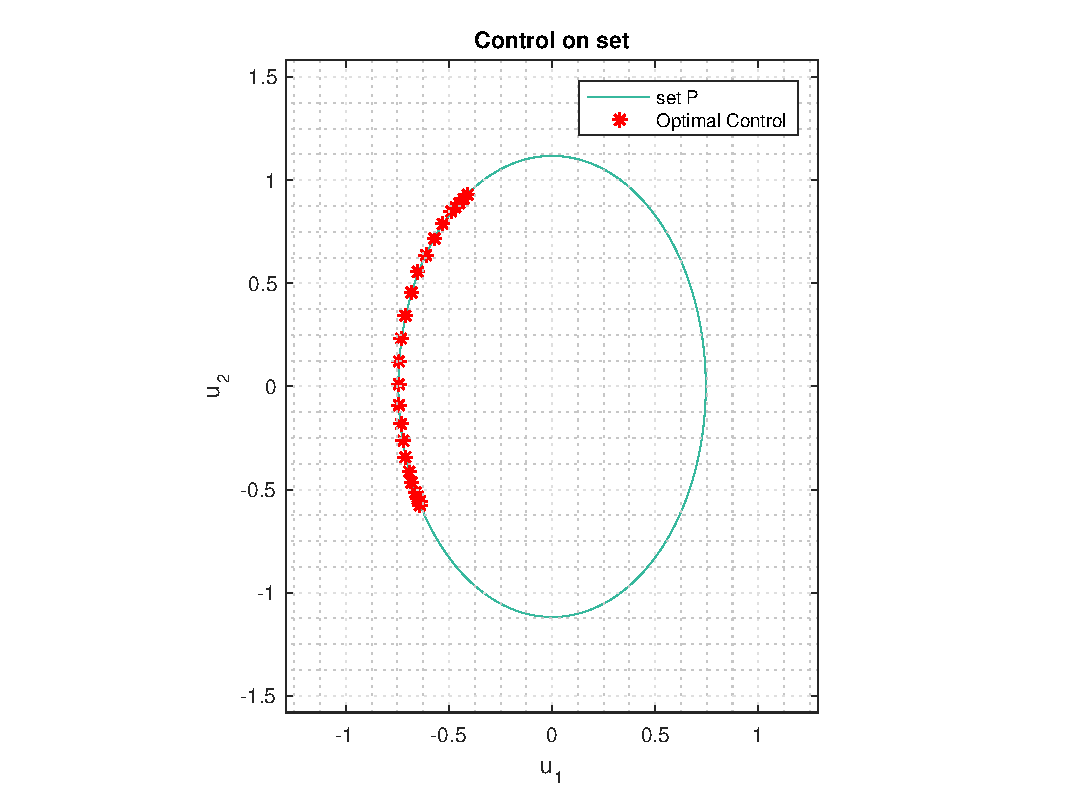
\includegraphics[width=\linewidth]{s4fig4}
            \label{pic:s4:4}
            \caption{Оптимальное управление на множестве \(\mathcal{P}\)}
        \end{subfigure}
        \caption{Оптимальное управление}
    \end{figure}
    \begin{figure}[H]
        \begin{subfigure}{0.5\linewidth}
            \centering
            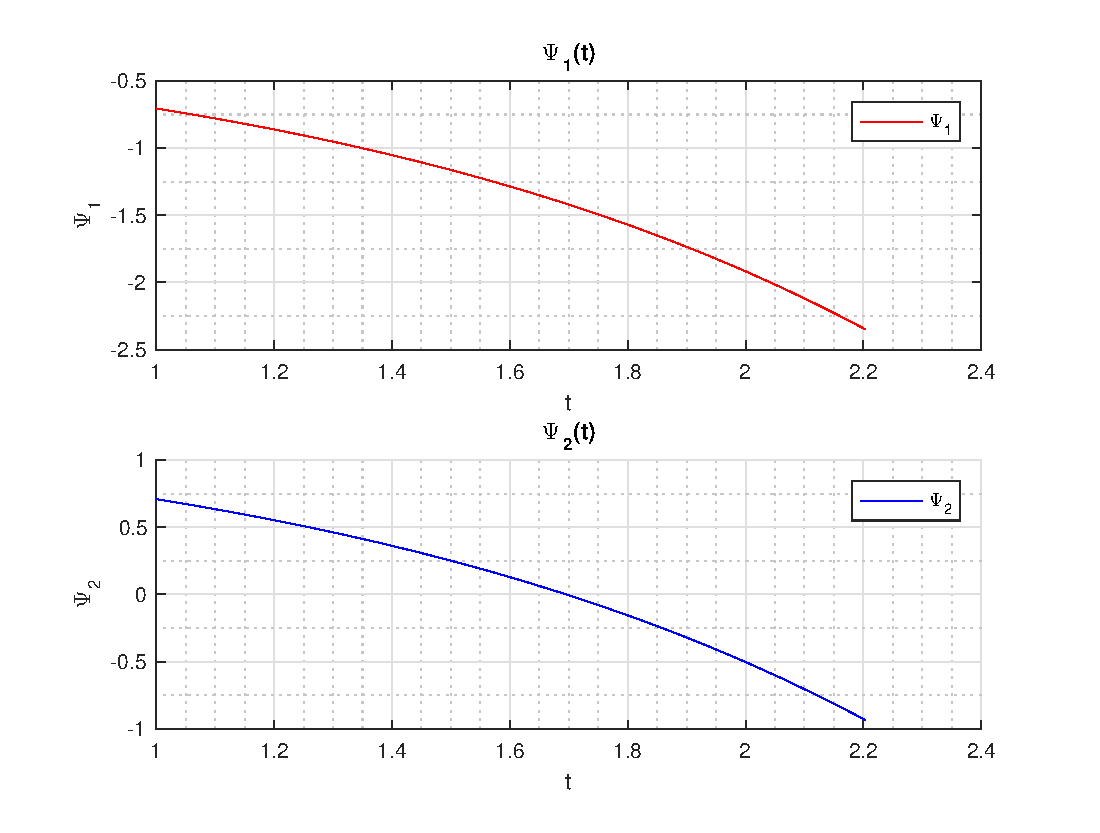
\includegraphics[width=\linewidth]{s4fig5}
            \label{pic:s4:5}
            \caption{Компоненты сопряжённых переменных}
        \end{subfigure}
        \begin{subfigure}{0.5\linewidth}
            \centering
            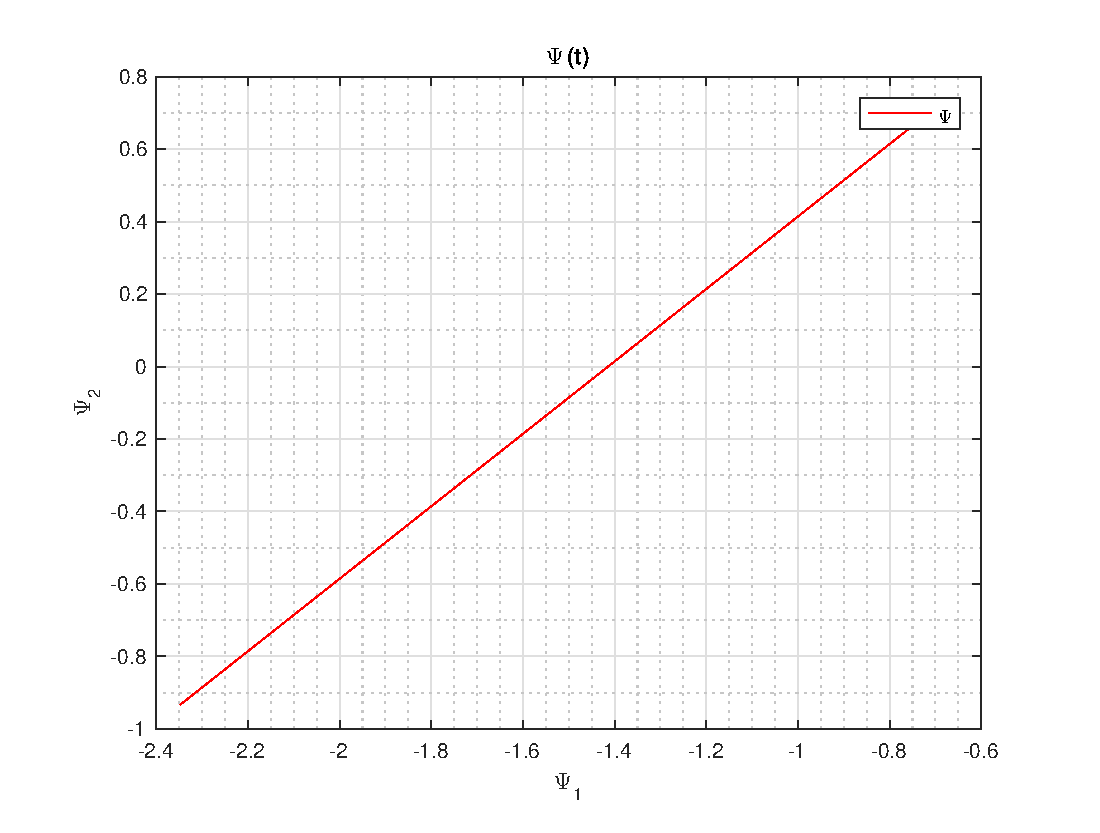
\includegraphics[width=\linewidth]{s4fig6}
            \label{pic:s4:6}
            \caption{Траектория сопряжённой системы}
        \end{subfigure}
        \caption{Сопряжённые переменные}
    \end{figure}
    % section code (end)
    \pagebreak
    \begin{thebibliography}{0}
        \addcontentsline{toc}{section}{Список литературы}
        \bibitem{Roublev:optimal:linear} И. В.~Рублёв. \emph{Лекционный курс Оптимальное Управление (Линейные Системы)},
        кафедра Системного~Анализа, Факультет Вычислительной Математики и Кибернетики, МГУ~им.~М.~В.~Ломоносова, 
        2017
        \bibitem{RoublevTochilin:matlab} Точилин~П.~А. \emph{Лекционный курс Программирование на языке \texttt{MATLAB}},
        кафедра Системного~Анализа, Факультет Вычислительной Математики и Кибернетики, МГУ~им.~М.~В.~Ломоносова, 
        2017~-- 2018
        \bibitem{Pontr'yaginEtAl:maximum} Понтрягин Л. С., Болтянский В. Г., Гамкрелидзе Р. В., Мищенко Е. Ф.~\emph{Математическая~теория~оптимальных~процессов}, — М.: Наука, 1976.
        \bibitem{Matlab:help} Справочные средства языка \texttt{MATLAB}
    \end{thebibliography}
\end{document}
